\documentclass{article}
%\usepackage{fullpage}
\usepackage{mathtools}
\usepackage{mhchem}
\usepackage{amssymb}
\usepackage{amsmath}
\usepackage{bm}
\usepackage{gensymb}
\usepackage{siunitx}
\usepackage{cancel}
\usepackage{graphicx}
\usepackage{subcaption}
\usepackage{mdframed}
\author{Mann, J}
\title{Day 12 Notes}
\date{October 6, 2015}
\newenvironment{aside}{\begin{mdframed}}{\end{mdframed}}
\renewcommand{\d}[0]{\mathrm{d}}
\newcommand{\pOne}[2]{\frac{\partial #1}{\partial #2}}
\renewcommand{\deg}[0]{\degree}
\newcommand{\pTwo}[2]{\frac{\partial^2 #1}{\partial #2^2}}
\newcommand{\dOne}[2]{\frac{\d #1}{\d #2}}
\newcommand{\dTwo}[2]{\frac{\d^2 #1}{\d #2^2}}
\newcommand{\diag}[1]{\bcancel{#1}}
\newcommand{\matr}[1]{\bm{#1}}
\newcommand{\note}[1]{\vspace{3\parsep}\textit{\textbf{Note: }}#1\vspace{2\parsep}}
\newcommand{\norm}[1]{\left|#1\right|}
\newcommand{\aistar}[0]{\vec{a}_i^\ast}
\newcommand{\ai}[0]{\vec{a}_i}
\newcommand{\aone}[0]{\vec{a}_1}
\newcommand{\atwo}[0]{\vec{a}_2}
\newcommand{\bone}[0]{\vec{b}_1}
\newcommand{\btwo}[0]{\vec{b}_2}
\newcommand{\nvec}[0]{\vec{n}}
\newcommand{\pmat}[1]{\begin{pmatrix}#1\end{pmatrix}}
\newcommand{\qvec}[0]{\vec{q}}
\newcommand{\xvec}[0]{\vec{x}}
\graphicspath{{Day12NotesPics/}}
\begin{document}
\maketitle{}
\begin{section}{Intro}
	\begin{itemize}
		\item Questions on the problem set
		\item Matrix method of constructing $\vec{a}_i^\ast$ from $\vec{a}_i$
		\item Adsorption on surfaces - some structure considerations
		\item Symmetry considerations
	\end{itemize}
\end{section}
\begin{section}{Diffraction methods - Examples}
The data that you see is encoded on the screen, and you can determine positions (and therefore angles and wave numbers) quite accurately.
Example
\begin{figure}[h]
	\centering
	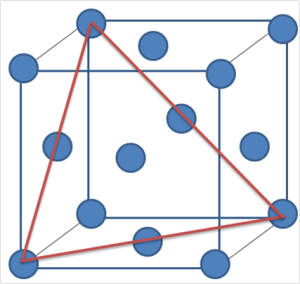
\includegraphics[height=100pt]{FCC111}
	\caption{Face centered cubic, such as platinum. We show the (111) direction}
	\label{fig:FCC}
\end{figure}

Now picture the unit ``mesh''. Such as Figure~\ref{fig:unitMesh}
\begin{figure}[h]
	\centering
	
\includegraphics[height=100pt]{vacuumChamber}
	\caption{A unit mesh. Smiley faces are inserted until a better figure is available.} 
	\label{fig:unitMesh}
\end{figure}
Construct $\aone$ and $\atwo$.

\begin{align*}
	\aone = \frac{1}{\sqrt{2}}a(1,0)\\
	\atwo = \matr{Q}\cdot \aone
\end{align*}
where $a$ is a literature value, and $\matr{Q}$ is a rotation matrix.
\begin{align*}
	\matr{Q} = \begin{pmatrix}\cos\theta & -\sin\theta\\\sin\theta & \cos\theta\end{pmatrix}\\
	\begin{pmatrix}\cos\theta & -\sin\theta\\\sin\theta & \cos\theta\end{pmatrix}\begin{pmatrix}\cos\theta & \sin\theta\\-\sin\theta & \cos\theta\end{pmatrix} = \begin{pmatrix}1&0\\0&1\end{pmatrix}
\end{align*}
So $\matr{Q}$ is an orthogonal matrix, and
\begin{align*}
	\atwo = \matr{Q} (120^\circ)\aone
\end{align*}
$\norm{\aone\times\atwo}$ = \text{area of the mesh}

generate $\aone^\ast$, $\atwo^\ast$
Conditions:
\begin{align*}
	\vec{a}_i \cdot \vec{a}_j = \begin{cases}2\pi & i=j\\0 & i\neq j\end{cases}
\end{align*}
This comes from the diffraction physics, $\phi$.

Easier to normalize to 1, but don't forget $2\pi$ in the $\phi$ formulas.

Last time: Used the cross product ($\times$).
\begin{align*}
	\aone,\atwo,\nvec = \aone\times\atwo
\end{align*}
Now we use a matrix method
Surface of Pt(hkl).
Surface adsorption
Pt(hkl) Matrix adsorption

From the viewpoint of catalysis, you need to know
\begin{enumerate}
	\item Structure of the catalytic surface
	\item Structure of the adsorbed layer
	\item Chemical bonding that can occur
\end{enumerate}

Prior to 1955, the surface of the catalyst itself was a black box. You could look at adsorption isotherms, but without electron diffraction, you couldn't look at the surface itself.

You start out by constructing a matrix
\begin{align*}
	\matr{A} = \pmat{\aone\\\atwo} = \pmat{\vec{a}_{11} & \vec{a}_{12}\\\vec{a}_{21} & \vec{a}_{22}}
\end{align*}
Then you want $\aistar$ constructed from $\matr{A}^{-1}$
\begin{align*}
	\matr{A}^{-1} = \frac{1}{\det{\matr{A}}}\pmat{a_{22} & -a_{12}\\-a_{21} & a_{11}}
\end{align*}
But you should generally just use software to calculate the inverse of $\matr{A}$, $\matr{A}^{-1}$

$\matr{A}^{-1} = \frac{1}{\det{\matr{A}}}\pmat{a_{22} & -a_{12}\\-a_{21} & a_{11}} = \frac{1}{\det\matr{A}}\pmat{\vec{a}_1^\ast & \vec{a}_2^\ast}$
Show that 
\begin{align*}
	\aone \cdot \aone = \dots
\end{align*}

Now 
\begin{align*}
	\xvec_n = m_1\aone + m_2\atwo\\
	\qvec_n = k\aone^\ast + k\atwo^\ast
\end{align*}

This characterizes fully the substrate.

Suppose you have a powder of catalyst crystals:

\begin{figure}[h]
	\centering
	
\includegraphics[height=100pt]{vacuumChamber}
	\caption{By putting the catalyst into an evacuated weigh chamber, and controlling the vapor that goes in, you can get a plot of the $\Gamma$ vs $P/P_0$. The first plateau is monolayer adsorption, while the next would be multilayer adsorption.}
	\label{fig:catalystCrystals}
\end{figure}

You can weigh monolayers of material using this setup.

What is a bit crucial to know is a Brunaeur, Emmett and Teller isotherm. This isotherm is quite effective as long as you know the problems with the isotherm. This uses an unfounded assumption about the multilayer adsorption.

By and large, data quoting BET isotherms should be used with caution. Statistical mechanics is used now to generate the properties of true isotherms.

\begin{figure}[h]
	\centering
	
\includegraphics[height=100pt]{vacuumChamber}
	\caption{Square Lattice. There are several symmetry properties you should notice. One is translational symmetry. The x's denote molecules adsorbed on the surface. When you have things adsorbing on the surface, a rule of thumb is that it goes in the position of highest symmetry.}
	\label{fig:squareLattice}
\end{figure}
In the example of Figure~\ref{fig:squareLattice},$\aone,\atwo$ and $\vec{b}_1,\vec{b}_2$ are clearly related.
Kinds of symmetry
\begin{itemize}
	\item Translational: Obtained by moving the net over in a given direction. Not all surfaces have translational symmetry, which can affect the way a catalyst works.
	\item Rotational: Rotation by some angle $\theta$ will yield the original lattice.
	\item 
\end{itemize}

\begin{align*}
	\matr{A} = \pmat{\aone\\\atwo}\\
	\matr{B} = \pmat{\bone\\\btwo}\\
	\matr{B} = \matr{G}\cdot\matr{A}\\
	\matr{B}\cdot\matr{A}^{-1}=\matr{G}
\end{align*}

But, so much of the LEED data gives you $\matr{B}^\ast$ and $\matr{A}^\ast$. So you need to recognize that
\begin{align*}
	\matr{B}^\ast = \matr{G}^\ast\cdot \matr{A}^\ast
\end{align*}

You need to be careful about ordering of $\vec{a}_i$ in $\matr{A}$, $\vec{a}_i^\ast$ in $\matr{A}^\ast$, as well as  $\vec{b}_i$ in $\matr{B}$, $\vec{b}_i^\ast$ in $\matr{B}^\ast$, 

Algebra

\begin{align*}
	\matr{I} = \matr{B}\cdot\matr{B}^\ast\\
	\matr{I} = (\matr{G}\cdot\matr{A})\cdot(\matr{G}^\ast\cdot\matr{A}^\ast)^t\\
	\matr{I} = (\matr{G}\cdot\matr{A})\cdot\matr{A}^\ast\cdot\matr{G}^\ast\\
	 = \matr{G}\cdot\matr{G}^\ast
\end{align*}
The $t$ is so that you have the correct ordering.

Now be careful. For the algebra to work out, you want

\begin{align*}
	\matr{G}^\ast = (\matr{G}^t)^{-1},\matr{G} = (\matr{G}^{\ast t})^{-1}
\end{align*}

I'm following the usual way that this is presented. There must be a cleaner way of keeping track. Recognize that the problem of keeping track of whether it's
$\pmat{\aone&\atwo}$ or $\pmat{\aone\\\atwo}$ for $\matr{A}$, and for the other matrices as well.

The point is that $\matr{A}$ and $\matr{B}$ are related through $\matr{G}$ and $\matr{A}^\ast$, $\matr{B}^\ast$ through $\matr{G}^\ast$

Next time examples in terms of Wood's notation and the matrix notation.
\end{section}
\end{document}
